\section{Przegląd literatury - dostępne porównania baz danych}

 W~rozdziale zostały przedstawione dostępne porównania szybkości niektórych baz danych. Przytoczone porównania są w~pewnym stopniu punktem odniesienia do uzyskanych w~pracy wyników. W~każdym z~przypadków uzyskane wyniki są inne, testy były przeprowadzane na różnych danych. Różna była też ilość danych i~ich złożoność, a~także sposób implementacji bibliotek. 

\subsection{Core Data i~SQLite - porównanie wydajności}

Porównanie zaczerpnięte z~witryny internetowej http://www.drdobbs.com. Autor stworzył przykładową aplikację pozwalająca przeprowadzić operacje na głównych bazach danych iOS. Testy zostały przeprowadzone na iPhone 5s. \par

Do testów został użyty prosty zestaw danych, który jest widoczny na rysunku 3.1 znajdującym się poniżej. 

\begin{figure}[h]
	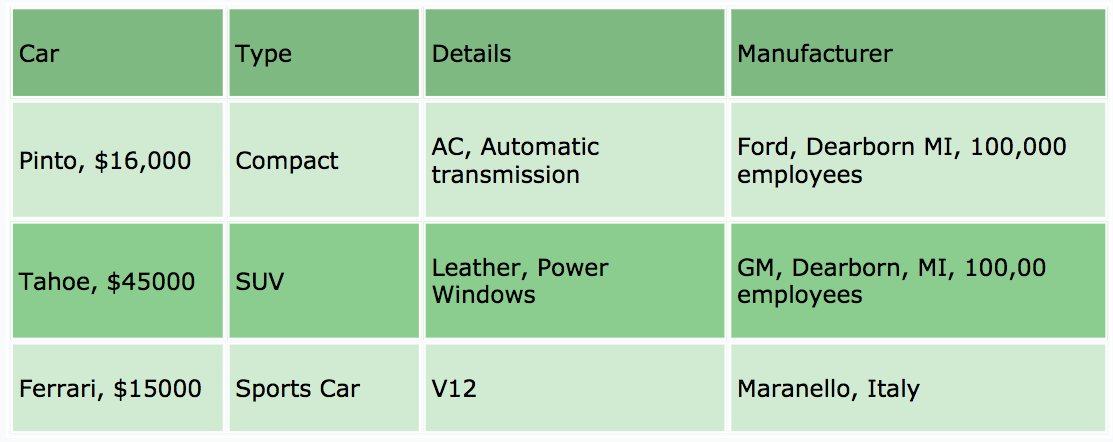
\includegraphics[width=\linewidth]{img/coredata_sql_test.png}
	\caption{Przykład danych użytych do porównania wydajności Core Data i~SQLite}
	\label{fig: CoreData_SQLite_test_data}
\end{figure}

%\begin{table}[]
%\begin{tabular}{|c|c|c|c|}
%\hline
%\rowcolor[HTML]{72B076} 
%Car              & Type       & Details                                                               & Manufacturer                                                                    \\ \hline
%\rowcolor[HTML]{CAE8CC} 
%Pinto, \$16,000  & Compact    & \begin{tabular}[c]{@{}c@{}}AC, \\ Automatic transmission\end{tabular} & \begin{tabular}[c]{@{}c@{}}Ford, Dearborn MI, 100,000 \\ employees\end{tabular} \\ \hline
%\rowcolor[HTML]{72B076} 
%Tahoe, \$45000   & SUV        & \begin{tabular}[c]{@{}c@{}}Leather, \\ Power Windows\end{tabular}     & \begin{tabular}[c]{@{}c@{}}GM, Dearborn, MI, 100,00 \\ employees\end{tabular}   \\ \hline
%\rowcolor[HTML]{CAE8CC} 
%Ferrari, \$15000 & Sports Car & V12                                                                   & Maranello, Italy                                                                \\ \hline
%\end{tabular}
%\end{table}

Autor przeprowadził testy pokazujące zajętość pamięci obiektu bazy na dysku urządzenia, testy użycia pamięci aplikacji używającej bazy oraz testy szybkości bazy podczas pobierania danych z~bazy. Poniższe rysunki 3.2, 3.3, 3.4 prezentują ich rezultaty.

\begin{figure}
\centering
	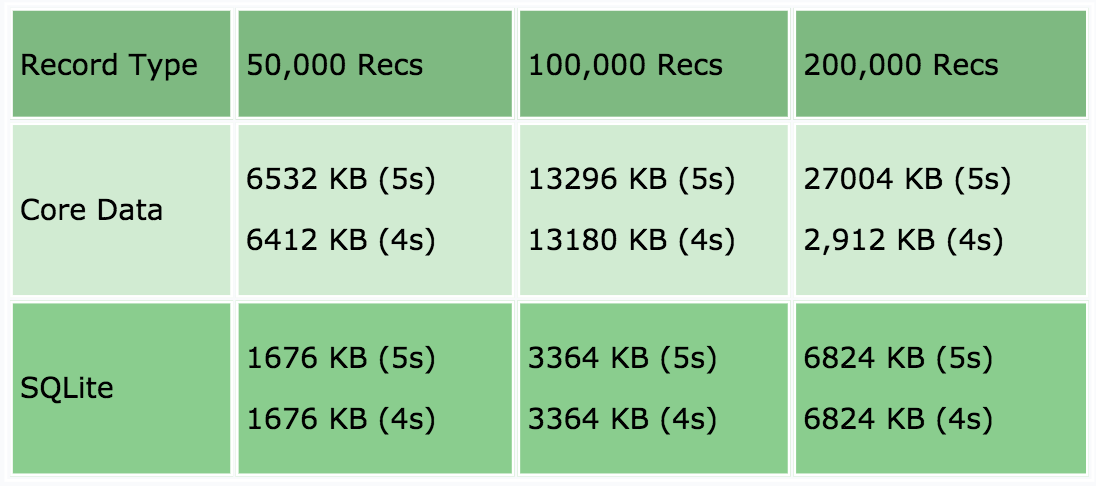
\includegraphics[width=13cm]{img/drdobbs_storage_test.png}
	\caption{Rezultat testów porównania Core Data i~SQLite - wielkość pliku bazy }
	\label{fig: CoreData_SQLite_storage_test}
\end{figure}

\begin{figure}
\centering
	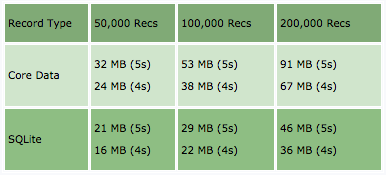
\includegraphics[width=13cm]{img/drdobbs_memory_test.png}
	\caption{Rezultat testów porównania Core Data i~SQLite - pamięć aplikacji}
	\label{fig: CoreData_SQLite_memory_test}
\end{figure}

\begin{figure}
\centering
	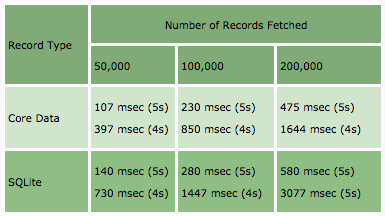
\includegraphics[width=13cm]{img/drdobbs_speed_test.png}
	\caption{Rezultat testów porównania Core Data i~SQLite - prędkość odczytu danych}
	\label{fig: CoreData_SQLite_speed_test}
\end{figure}
\clearpage

Wyniki wielkości pliku bazy pokazują, że plik bazy Core Data zajmuje około cztery razy więcej miejsca niż plik bazy SQLite. Na rysunku 3.3 widać, że Core Data zużywa też więcej pamięci operacyjnej podczas działania aplikacji. Autor tłumaczy, że wynika to ze sposobu, w~jaki działa Core Data. Tworzy ona w~pierwszej kolejności obiekty w~pamięci, a~dopiero później następuje zapis do bazy, przez co Core Data zużywa od 40\% do 100\% pamięci więcej niż SQLite. Rysunek 3.4 przedstawia czasy, w~jakich następuje kolejno odczyt 50 000, 100 000, 200 000 tysięcy rekordów z~baz. W~tym porównaniu znacząco dominuje Core Data. Na iPhone 4s osiąga dwukrotną szybkość odczytu danych. 

\subsection{Realm}

Wydawca Realm udostępnia na swojej stronie porównanie swojego rozwiązania z~bazami takimi jak: SQLite, FMDB, Core Data, Couchbase Lite, YapDatabase. W~testach zostały porównane prędkości zapisu danych, wykonania czasu zapytania oraz zliczenia rekordów. Poniższe rysunki pokazują ich wyniki. \par

\begin{figure}[h]
\centering
	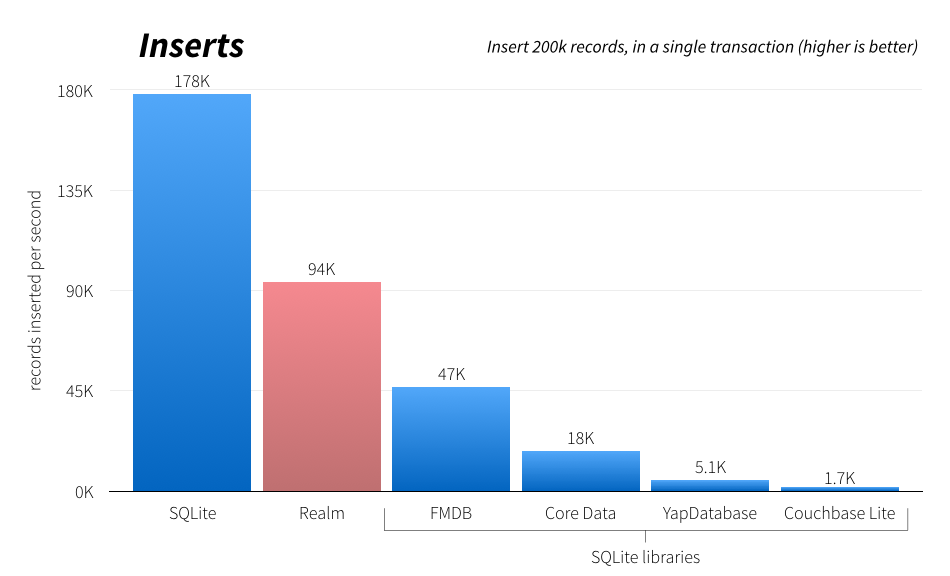
\includegraphics[width=\linewidth]{img/realm_insert_test.png}
	\caption{Rezultat testów Realm - zapis danych do bazy}
	\label{fig: realm_insert_test}
\end{figure}

\begin{figure}
\centering
	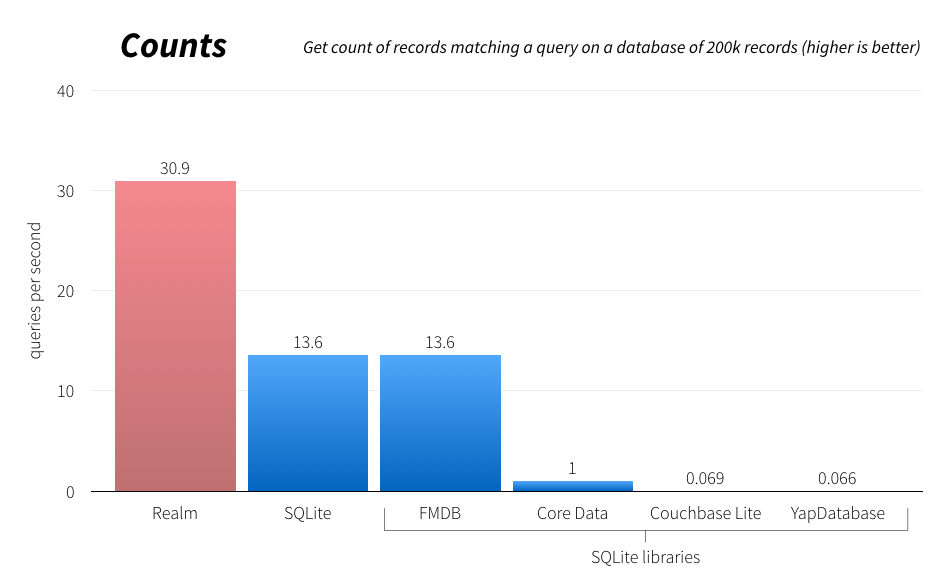
\includegraphics[width=\linewidth]{img/realm_count_test.png}
	\caption{Rezultat testów Realm - zliczanie rekordów}
	\label{fig: realm_count_test}
\end{figure}

\begin{figure}
\centering
	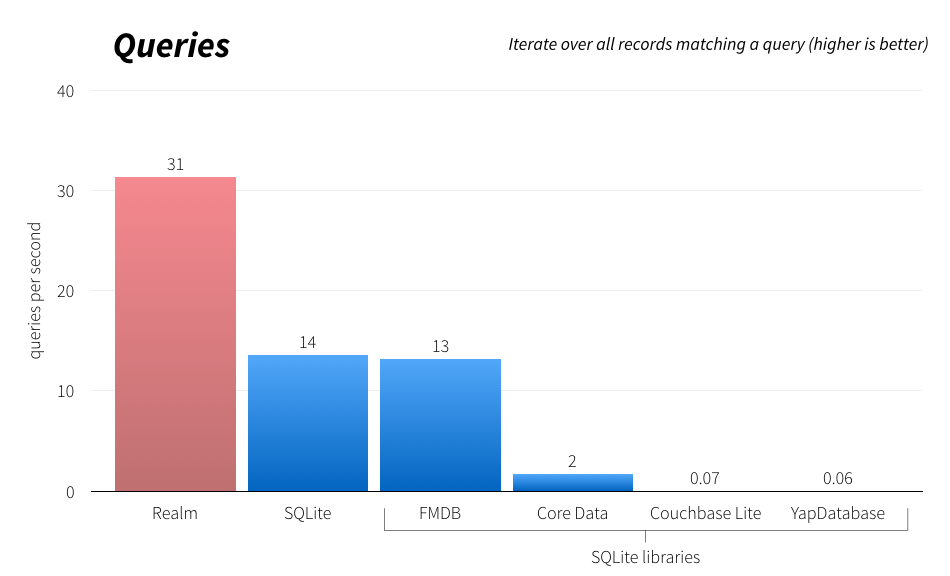
\includegraphics[width=\linewidth]{img/realm_query_test.png}
	\caption{Rezultat testów Realm - odczyt danych}
	\label{fig: realm_query_test}
\end{figure}
\clearpage

Realm w~opisach zapewnia, że ich produkt posiada doskonałą wydajność. Szybszą nawet w~niektórych przypadkach od SQLite. Testy wydają się potwierdzać ich słowa. SQLite wypadł gorzej od Realm tylko w~jednym teście, które przedstawili. Okazał się on najszybszy przy zapisie danych do bazy, osiągając blisko dwukrotnie wyższy wynik od Realm wynoszący 178 000 zapisanych rekordów w~ciągu sekundy, rezultat widoczny jest na rysunku 3.5. Kolejne testy pokazują dominacje Realm. W~teście zliczania rekordów SQLite i~FMDB uzyskują taki sam wynik - 13.6 operacji na sekundę zaś Realm wykonuje aż 30.9 operacji, co jest wynikiem ponad dwukrotnie wyższym. W~przypadku odczytu danych Realm też jest najszybszy. Osiąga wynik 31 operacji na sekundę, a~SQLite i~FMDB jedynie 13-14 operacji. Wynik kolejny raz jest ponad dwukrotnie lepszy. \par 
Wynik testów są bardzo imponujące i~dowodzą, że Realm jest jedną z~najszybszych baz danych. Autorzy testów niestety nie pokazują sposobu testowania baz ani nie ujawniają, na danych jakiego typu odbyły się testy.